
%----------------------------------------------------------------------------------------
%   PACKAGES & CONFIGURATIONS DU DOCUMENT
%----------------------------------------------------------------------------------------

\documentclass[12pt]{article}
\usepackage[english]{babel}
\usepackage[utf8x]{inputenc}
\usepackage{amsmath}
\usepackage{graphicx}
\usepackage{float}
\usepackage{fancyhdr}
\usepackage[toc,page]{appendix}
\renewcommand\appendixpagename{Appendix}
\renewcommand\appendixtocname{Appendix}
\usepackage[textwidth=17cm,textheight=22cm]{geometry}
\usepackage[colorinlistoftodos]{todonotes}


%----------------------------------------------------------------------------------------
%   HEADER
%----------------------------------------------------------------------------------------
\pagestyle{fancy}
\renewcommand\headrulewidth{1pt}
\fancyhead[L]{RICM4}
\fancyhead[R]{Polytech Grenoble}

\begin{document}

\begin{titlepage}

\newcommand{\HRule}{\rule{\linewidth}{0.2mm}} % Commande définie pour les lignes horizontales (changer l'épaisseur ici)

\center % Centre tout sur la page
 
%----------------------------------------------------------------------------------------
%   TITRES
%----------------------------------------------------------------------------------------

\textsc{\LARGE Polytechnic school of Grenoble-Alpes university}\\[1.0cm] % Nom de l'université
\textsc{\Large RICM4}\\[1.5cm] % Nom de la filière

%----------------------------------------------------------------------------------------
%   TITRE PRINCIPAL
%----------------------------------------------------------------------------------------

\HRule \\[0.5cm]
{ \huge \bfseries Internship report}\\[0.2cm] % Titre du document
\HRule \\[1.5cm]
 
%----------------------------------------------------------------------------------------
%   AUTEUR & TUTEUR
%----------------------------------------------------------------------------------------

\begin{minipage}{0.47\textwidth}
\begin{flushleft} \large

\

\emph{Student :}\\
Julien \textsc{Cordat-Auclair} % Nom
\end{flushleft}
\end{minipage}
~
\begin{minipage}{0.47\textwidth}
\begin{flushright} \large

\

\emph{Supervisor :}\\
Sebastien \textsc{Pittion} % Nom du tuteur
\end{flushright}
\end{minipage}\\[3cm]

%----------------------------------------------------------------------------------------
%   DATE
%----------------------------------------------------------------------------------------

{\large 13 August 2018}\\[4cm] % Date

%----------------------------------------------------------------------------------------
%   LOGO
%----------------------------------------------------------------------------------------


\includegraphics[scale=0.25]{logoUGA.png}\\[1cm] % Logo de l'université
 
%----------------------------------------------------------------------------------------

\vfill % Remplir le reste de la page avec des lignes vides

\end{titlepage}

%----------------------------------------------------------------------------------------
%   PLAN
%----------------------------------------------------------------------------------------

\renewcommand{\contentsname}{Table of content}

\tableofcontents{}

%----------------------------------------------------------------------------------------
%   RAPPORT
%----------------------------------------------------------------------------------------

%   REMERCIEMENTS

\newpage
\section{Acknowledgement}

Before starting this internship report, I would like to thank Mr. Christian Pomot (director of Com\&Net) who accepted to welcome me into his company and who taught me a lot during these 12 weeks by transforming this professional experience into a moment both extremely rewarding and very profitable. He was always available and at listening when I encountered any kind of difficulty, and talking with him allowed me to find a logical solution to each of them.

\

I also thank my supervisor who has regularly assisted me throughout this period with a lot of pedagogy and who has always been available in case of problem. Finally, I would like to thank all the company's employees for their feedback as well as Théo Echevet (student in RICM4) who has helped me several times, without forgetting Mr. Christophe Brouard (researcher at the Laboratoire Informatique of Grenoble) for his help during this project.
\

\

%   INTRODUCTION

\newpage
\section{Introduction}

\subsection{Context}

From May 21 to August 13, I did an internship at \textsc{Com\&Net}. This company specialized in the web allows its customers to develop their websites while optimizing their SEO. During this period, I worked in the company's offices in Grenoble and was accompanied by \textbf{M. Christophe Pomot} (director), two employees, an alternate and \textbf{Théo Echevet}. The company manager provided me clear and precise specifications for the project he had assigned to me, the main requirement being the use of \textbf{M. Christophe Brouard}'s algorithm.

\

\subsection{Mission}

During this internship, I had to set up a service to submit recommendations to a user regarding the referencing of his web page for a given request. The user therefore provides the URL of his page as well as the keywords for which he wants it to be referenced at the best and the service must send him a set of information helping him to achieve this objective. This application also uses the machine learning algorithms developed by \textbf{M. Christophe Brouard} called \texttt{Echo}. The project is therefore distinguished in three specific steps: data collection from the web, machine learning from it and then displaying the results returned by \texttt{Echo}. 

\

The project therefore raises back-end and front-end issues, establishing a rich and complete field of study, especially since multiple languages, frameworks and libraries have been used: \textsf{Python}, \textsf{PHP}, \textsf{HTML}, \textsf{CSS}, \textsf{JavaScript} and \textsf{Scrapy} (\textit{scrapy.org}), \textsf{Selenium} (\textit{www.seleniumhq.org}), \textsf{Symfony} (\textit{symfony.com}), \textsf{jQuery} (\textit{jquery.com}) or the template engine \textsf{Twig} (\textit{twig.symfony.com}). In addition, it is important to note that the service I have implemented will be used later by the company to facilitate SEO tasks, both for customers and employees specialized in this field who will then have an additional tool at their disposal to perform this important work when it comes to establishing an effective digital strategy. 

\

Finally, the efficiency of this service must be optimal in order to be able to propose modifications that will allow the sites analysed to gain as many places as possible: it should be noted that only the 3 best positioned pages attract the attention of users, the others going almost unnoticed (only 10\% of attention is given to them). The problem of referencing is therefore essential for any person or company wishing to stand out from the others and the interest shown in it can only increase over time.

\

\

\

Here are two tables to illustrate this project; the first presents the parameters entered by the user and the second corresponds to the results that will be returned to him:

\

\begin{center}
\begin{tabular}{|c|c|}
\hline
user's URL & http://com-et-net.com \\
\hline
keywords & stratégie numérique grenoble \\
\hline
\end{tabular}

\

\

\begin{tabular}{|c|c|c|}
\hline
\texttt{EchoBT} & référencement\_title, agence\_title, stratégie\_alt, isère\_strong ... \\
\hline
\texttt{EchoPos} & 14 \\
\hline
\texttt{EchoV} & 0.76, 0.63 \\
\hline
\end{tabular}
\end{center}

\

All these information will be explained later.

\

\subsection{Plan}

As stated earlier, three obvious steps have emerged during this project and will form the outline of this report. As a reminder, the first was a web scraping step (data collection from the internet), then came the machine learning (processing of these data) to finally give way to UX Design (optimization of the display of results). However, a presentation of the company in which I have worked is necessary before looking at the work done over the past three months.


%   COM&NET

\newpage
\section{\textsc{Com\&Net}}

\subsection{Presentation of the company}

\textsc{Com\&Net} was called \textsc{Mountain\&Net} until 2016. Founded in 2003 by \textbf{M. Christian Pomot}, this company is focused on the creation of web tools specific to tourism professionals, particularly in the Vercors region in which it was previously located. Today, \textsc{Com\&Net} has strengthened its presence in Grenoble by setting up offices there, but it still maintains an antenna in Villard-de-Lans to be able to remain close to its former customers. It is indeed in this city that the company was initially created and it is here that it has been able to develop.

\

The company thus supports the projects and the presence on the internet of various tourist structures such as hotels, resorts or other activities. Its main assets are obviously the mastery of the IT field but also an excellent approach to the various issues related to tourism. It offers different types of services such as website creation, SEO optimization, promotion and application development.

\

\subsection{Website and application development}

The company masters a wide range of frameworks in order to best adapt to the needs of its customers. \textsf{Symfony} (a \textsf{PHP} framework allowing a structured and fast development) and \textsf{Copix} are the most used in the case of large projects. \textsf{Thelia} (an Open Source solution that appeared in 2006) is also a framework that employees are able to use when setting up an e-commerce site. Thus, the company develops many tourist sites but also applications such as \textsc{GTE} which allows the traceability of explosives for winter sports resorts.

\

In addition to their creation, \textsc{Com\&Net} also hosts and maintains the websites. Employees are always available to answer any questions from customers and are ready to solve any problems at any time.

\

\subsection{Digital strategy}

\textsc{Com\&Net} is also a company specialized in digital strategy, i.e. the different methods used to optimize the visibility of its clients' websites in search engine results. It is partly with this in mind that a partnership was set up with the \textsc{Grenoble Alpes university} in 2015 to be able to use the machine learning algorithms developed by \textbf{M. Christophe Brouard}.

\

\subsection{Organisation}

\textsc{Com\&Net} is a \textsf{SARL} (Limited Liability Company), which means that there is a single partner, in this case \textbf{M. Christian Pomot}. Three people are employed in the company and currently accompanied by an alternate (see \textsl{appendix 1}). Two sectors are clearly distinguished within it: the first is dedicated to the development of websites and applications, the second is dedicated to digital strategy and web marketing.

\

\subsection{Sustainable development}

To reduce its carbon footprint, \textsc{Com\&Net} has chosen to have its various servers hosted by \textsc{PHPNET}. The eco-responsible approaches that this Grenoble company offers are as follows:
\begin{itemize}
	\item the use of SSD servers offering optimal reliability and a significant reduction in power consumption (nearly 98\% less energy than traditionally)
	\item the donation of old computer equipment to the association \textit{Ulisse Solidura} with a view to recycling through their workshop named \textit{DEEE} (Waste Electrical and Electronic Equipment)
	\item the use of so-called Free Cooling technologies designating natural cooling and thus allowing the company's datacenter to be cooled by outside air if its temperature is lower than that of the inside (therefore very practical in winter)
	\item the connection of the data centers to the Grenoble power grid \textsc{GEG} (green electricity)
	\item hosting of servers for associations such as \textit{Les Jardins de la Solidarité}, an integration project combining organic market gardening, a nursery and green spaces
\end{itemize}

\

In addition, \textsc{Com\&Net} uses \textsc{Terra} computers to reduce power consumption due to computer equipment. These are certified by the \textsc{Energy Star 5.0} and therefore have low energy consumption. The company therefore reduces energy consumption in addition to greenhouse gas emissions. \textsc{Terra} also optimizes its computers a little more over time (about 35\% reduction in consumption between current devices and devices that are 3 years old). The screens are also chosen by this brand, implying an even greater overall reduction in energy consumption.

\

Finally, it is important to note that \textbf{Christian Pomot} owns an electric car and is far from insensitive to sustainable development. Trainees and alternates who have had the opportunity to work in the company's offices in Grenoble have always traveled by tram or on foot.

%   1ERE PARTIE : WEB SCRAPING

\newpage
\section{First part: web scraping}

\textit{Before any development, a diagram representing the general architecture of this step and the links between the different files that compose it is available (see \textsl{appendix 2}).}

\subsection{General overview}

The first phase of this project focused on data recovery from the web. As the internship is focused on the theme of machine learning, it seems essential to be able to provide elements to the machine learning algorithm in order for it to work. As the purpose of the service is to optimize the referencing of a web page, the idea is to focus on public data related to this domain. This step consists in collecting the content of the tags that weigh on the balance of the referencing of a web page, and this for a significant number of sites displayed following a Google request (this request being chosen by the user). We then speak of SEO On-Site (SEO stands for Search Engine Optimization, On-Site designating all the SEO optimization actions that take place on the website and its contents). The positioning of the user's site cannot be optimized in the most efficient way thanks to this method since the Off-Site SEO (everything related to the very structure of the site) is not supported by the service. However, it is an improvement that the director of Com\&Net is strongly considering as part of the continuation of this project in order to obtain a complete but above all very efficient tool.

\

To do this web scraping work, \textbf{M. Christian Pomot} insisted that I use the language \textsf{Python} as well as the \textsf{Selenium} and \textsf{Scrapy} frameworks; the first one simulates a web browser and the "human" interactions that go with it (like a mouse click or a pressed keyboard key) and the second one makes it possible to create indexing robots capable of performing web scraping tasks (ie. retrieve data \textsf{HTML}). Their combination therefore seems perfectly adapted to the project.

\


\subsection{Description of the work performed}

\subsubsection{Retrieving URLs}

First, I used \textsf{Selenium} to be able to generate a Google query based on the keywords entered by the user. These keywords, as well as the URL of the latter's web page, are actually stored in a text file (with other parameters) and the web scraping engine is able to extract them. In this way, the retrieval of URLs and the entire process that follows will be adapted to the user's request. The product text file is interpreted as follows: 

\begin{center}
 \begin{tabular}{|c|c|c|c|}
\hline
1st line  & user's URL \\
\hline
2nd line & number of pages to be studied \\
\hline
3rd line & degree of pertinence \\
\hline
following lines & keywords \\
\hline
\end{tabular}
\end{center}

\

The idea is to retrieve the URLs present on the results page of the user request in order to extract the data that interests us. A Google search link can be written: \texttt{https://www.google.com/search?q=keyword1+keyword2+keyword3}. You simply have to change the keywords of this link to those chosen by the user to be able to display the desired results page using the functions offered by \textsf{Selenium}. 

\

In addition, Google displays 10 results per query by default. This value can be modified (up to 100) and it was interesting to be able to vary this number, which determines the quantity of URLs, and therefore potential data, to be analyzed later. I then added the suffix \texttt{\&num=100} to the search link to display 100 results. And if you want to retrieve more than 100 URLs, then the script is able to make a first request where it looks for the first 100 and then generate a new request with the suffix \texttt{\&sa=N} telling Google to display the second page. Then, it is necessary to identify in the source code of the results page the tags that identify the presence of a link to a web page. Again, a function of texttsf{ Selenium} allows to retrieve the content of the identified tag. This is how the script is able to return a list of URLs classified by position from a set of keywords and a given number of results.

\

\subsubsection{HTML data collection}
 
Secondly, \textsf{Scrapy} helped me to save the SEO data for each of the URLs I had previously found. Once the script involving \textsf{Selenium} has been executed, it is sufficient to provide the list of URLs to \textsf{Scrapy} so that the latter can analyze them. So during this step I specified the different important tags for SEO in order to extract the content for each web page previously returned. Thus, the tags \textit{title}, \textit{h1}, \textit{h2}, \textit{h3}, \textit{strong}, \textit{a}, \textit{p} and the attribute \textit{alt} of the tag \textit{img} and the words appearing in the URL of the site (after the domain name) were retained. According to \textbf{M. Christian Pomot} and the majority of studies published on the Internet, all these values are the ones that count for the referencing of a web page. However, Google does not confirm the veracity of these assumptions. On the other hand, it should be noted that the content that is part of the SEO On-Site changes regularly as evidenced by the tag \textit{keywords} which was essential a few years ago but no longer has any impact on SEO today. And it is very easy to adapt to these variations through the script described here since it is enough to manually change the tags to study. 
\

\textsf{Scrapy} finally allows to send back a \textsf{JSON}  file containing all the recovered data: it is this file that will later make the link with the machine learning step. This framework is very fast because it works asynchronously. However, this is a problem here since we necessarily lose the position given by the index of the page analyzed in the table of URLs previously returned. So I had to explicitly assign a position to each page to keep this information provided by \textsf{Selenium}.

\

\subsubsection{Link with machine learning}

Once the data has been retrieved, the idea is to be able to transmit it in any way to the machine learning algorithm. Knowing that this second major step (presented later) is coded in \textsf{PHP} within a \textsf{Symfony} project, it is essential to be able to provide from \textsf{Python} data that will be readable not only by \textsf{PHP} but also by the machine learning algorithm. The \textsf{PHP} language is able to read a \textsf{JSON} file, so no real modification is necessary on this point (except for some encoding problems) since it is the output format of the \textsf{Python} script. However, the algorithm developed by \textbf{Mr. Christophe Brouard} is not able to read any form of punctuation, accentuation or double, triple spaces, etc. It is therefore necessary to ensure that there is none as soon as possible. Before moving on to the next step, a complete cleaning of the data is therefore carried out.

%   2EME PARTIE : MACHINE LEARNING

\newpage
\section{Second part: machine learning}

\textit{Before any development, a diagram representing the general architecture of this step as well as the links between the different files of which it is composed is available (see \textsl{appendix 3}).}

\subsection{The Echo algorithm}

As stated above, this internship revolves around the theme of machine learning since the most important initial specification was the use of the machine learning algorithm (named \texttt{Echo}) developed by \textbf{M. Christophe Brouard}. In fact, in this project, three algorithms with specific actions and derived from \texttt{Echo} were used: \texttt{EchoBT}, \texttt{EchoV} and \texttt{EchoPos}.
\begin{itemize}
	\item \texttt{EchoBT} (\textit{BT} meaning \textit{best-terms}) allows, given a set of words each accompanied by an identifier and a relevance index, to determine which terms appear to be the best ones in order to improve referencing. Based on what was done in the previous step, the words will be the terms contained in each retrieved tag, the identifier will correspond to the name of the site associated with the current word and the relevance index will be a constant that will determine up to which position the sites are judged to be well referenced (for example, we can estimate that the 20 best referenced sites are relevant, so these sites will have a relevance index of 1 and all others will have a relevance index of 2 which corresponds to \textit{non relevant}). Thanks to these parameters, the algorithm will be able, via machine learning methods, to identify which terms are important for SEO by finding those that appear in relevant sites but not (or only slightly) in irrelevant sites. Note that \texttt{EchoBT} returns 30 terms ranked in descending order of score (from most effective to least effective), but this value can be modified to obtain more.
	\item \texttt{EchoV} (\textit{V} meaning \textit{verified}) allows with the same parameters as those of \texttt{EchoBT} to provide a performance rate representing the quality of the results returned by \texttt{EchoBT}. Indeed, it can sometimes be difficult to isolate effective terms for SEO (for example, if all the terms provided to \texttt{EchoBT} are identical, then the algorithm will not be able to find a term that appears in one of the relevant sites but is not present in an irrelevant site) and the performance rate will then be very low. Conversely, it may also be easy to know which term is \textit{SEO-efficient} (for example, if all relevant sites contain a common term and that term never appears in one of the sites deemed irrelevant), leading to a high performance rate.
	\item \texttt{EchoPos} (\textit{Pos} meaning \textit{position}) allows from the same parameters accompanied in addition to the content of the user's site as well as the keywords composing the Google query to estimate the position of the page provided for this query. In addition, a confidence rate is calculated to determine whether or not to rely on this result.
\end{itemize}

\

\subsection{Description of the work performed}

\subsubsection{Architecture of the Symfony project}

It is from this stage of the project that the framework \textsf{PHP} \textsf{Symfony} is used. In addition to linking data recovery to the display of results, the algorithms \texttt{Echo} must be called during the recovery. So it's probably the most important of the three. \textsf{Symfony} imposes a very particular architecture and allows to develop in MVC (\textit{Model-View-Controller}) in a fast, clean and efficient way. To make the most of this framework, I had to organize my project as follows: 
\begin{itemize}
	\item a first script (called \textit{controller} under \textsf{Symfony}) allows to recover the data: it then makes the link with the first step. In addition, it also generates the text file that contains the parameters of the study to be conducted and is used by the web scraping engine.  
	\item a second controller allows to execute the machine learning algorithms with these data: this is the second step. This is essential because it is at the origin of obtaining recommendations regarding content.
	\item a set of files \textsf{HTML}, \textsf{CSS} and \textsf{JavaScript} allows to display the returned results thanks to \textsf{jQuery} as well as successive calls \textsf{Ajax} (\textsf{Ajax} means \textit{Asynchronous JavaScript + XML} and allows to make requests \textsf{HTTP} into \textsf{JavaScript}). This is the third and final step and requires careful consideration because it requires displaying a lot of data while making it easier for the user to read.
\end{itemize}

\

\subsubsection{Data transmission}

The algorithms used \texttt{EchoBT}, \texttt{EchoV} and \texttt{EchoPos} need data to be able to work. The parameters provided by the user (keywords forming the Google query and page URL) are written in a text file and accompanied by the number of results desired and the degree of relevance. This configuration file is then sent to the script \textsf{Python} which will be executed. However, once the scraping data is retrieved from the \textsf{Symfony} project, prior processing is required before calling the algorithms. Indeed, the terms transmitted to the latter must keep the information related to the tag to which they are associated, otherwise terms of the tag \textit{title} could for example be compared to terms of the tag \textit{h3} and this would not make sense. That's why a suffix ''\_TITLE'' is added to a term in a tag \textit{title}, ''\_H3'' for a term in a tag \textit{h3}, etc. It will therefore be in this format that the data will be transmitted to the algorithms \texttt{Echo}. In addition, the contents of the relevant pages are duplicated a number of times and according to their actual position in the Google results page in order to give them more importance during the machine learning process.

\

\subsubsection{Echo calling and data recovery}

Each algorithm runs on a local TCP server with a different port number. Thus, it is enough to connect to the right port and transmit the necessary information to be able to execute the algorithm that interests us and retrieve the results provided.

\

Once the algorithms have analyzed the data, the results are returned to the \textsf{PHP} script. A function then allows you to sort the best terms provided by \texttt{EchoBT} both by tag importance (for example, the tag \textit{title} is more important to SEO than the tag \textit{strong}) and by score. This function also allows you to limit the number of terms to be displayed for the user; for example, you do not want to have 100 terms in the tag \textit{h3}. It will be these pre-processed data that will be posted later.

%   3EME PARTIE : UX DESIGN

\newpage
\section{Third part: results display}

\textit{Before any development, screenshots of the final display are available (see \textsl{appendices 4, 5, 6 and 7}).}

\subsection{General overview}

The last step of this project is dedicated to displaying the results previously returned by \texttt{Echo}. It implements issues related to UX Design (for \textit{User Experience Design}), the field of computing which consists in designing a website in the best possible way so that its use is optimal. Initially, the basic criteria for my project and for the user were as follows: 
\begin{itemize}
	\item he must be able to enter keywords (which form the Google query)
	\item he must be able to enter an URL (the one of the page he wants to optimize)
	\item he must be able to launch the study
	\item he must be able to visualize the results of this study
	\item he must be able to understand these results in order to benefit from them
\end{itemize}

\

\subsection{Description of the work performed}

\subsubsection{Data recovery}

Before wanting to process the display of results, it is necessary to be able to appropriate them. The link with the previous step is then made in \textsf{jQuery} thanks to \textsf{Ajax} calls which allow to retrieve the information returned by \texttt{Echo}. This method also allows each of the steps to be performed one after the other once the user decides to launch the study. This makes it easy to identify any problem if an error occurs during the process. Finally, the use of this structure ensures an optimal execution speed and therefore a minimum waiting time for the user since the different pages (loading and results) are loaded on site. 

\

\subsubsection{Results, display and user interface}

The third step focuses on optimizing the display of the results returned by \texttt{Echo} following learning from a data set provided by the script \textsf{Python}; these are diverse and varied and are composed of the following elements:
\begin{itemize}
	\item an integer with a percentage returned by \texttt{EchoPos} : they correspond respectively to the estimated position of the user's page in Google results for the given query and the confidence rate that can be given to this result.
	\item a percentage returned by \texttt{EchoV} : it corresponds to the performance rate of \texttt{EchoBT}. This allows the user to know how confident he or she can be in the results provided by the user.
	\item a set of \textit{n} terms of the form''word1\_BALISE'' where \textit{word1} corresponds to a word considered important with regard to SEO by \texttt{EchoBT} and \textit{BALISE} refers to the tag in which this term is located. The whole \textit{n} can be modified in the code.
\end{itemize}

\

I have decided to split the display into two distinct parts: at the very top of the page, the user will see first a section dedicated to general information about the study he has requested (see annex). This includes a summary of his research, the estimated position of his page, links to the best referenced sites for the given request without forgetting two graphs representing the percentages mentioned above. Tooltips accompany them in order to clearly translate their function.

\

Then, a second section displays the best terms returned by \texttt{EchoBT}. Each term is stored in a sub-section dedicated to the tag to which it is associated, and all terms present within the same sub-section are classified by decreasing order of score (a color code is used to reflect this). In addition, the subparts are displayed in order of importance of the corresponding tag: the terms of the tag \textit{title} appear at the top because it is the most important for SEO, but those of the attribute \textit{alt} appear lower because it is considered less effective.

\

\subsubsection{Additional features}

Each subpart is accompanied by a text field in which the content of the page to be optimized is written and which is associated with the corresponding tag. This field can be modified by the user: the idea is to write new relevant content using terms indicated above which, according to \texttt{Echo}, allow for better referencing. Each tag has its own field that can be freely modified. Once the modifications have been made, the user then gains access to two buttons at the bottom of the page: the first allows the position of the page to be recalculated with the modifications made and the second allows the changes to be exported as a \textsf{JSON} file.

%   BILAN

\newpage
\section{Summary}

\subsection{Analysis of the work carried out}

This project was complete and required a lot of thought with regard to its organization. First, it was necessary to code a web scraping engine using \textsf{Scrapy} and \textsf{Selenium}. This one is able to retrieve the HTML data contained in specific tags of the best referenced web pages for a given request; it was mainly intended to provide the necessary and cleaned data (accents, punctuation and unnecessary spaces) to \texttt{Echo} for machine learning. This central step of the internship allowed me to take charge of the \textsf{PHP Symfony} framework and I had to, during this one, find a way to make the link with the previous one while keeping the information related to the tag associated with each term. Finally, many issues related to the display of results and its ergonomics were raised, but this UX Design step finally resulted in something complete, clean and easy to read. Moreover, it was during this one that I was able to discover \textsf{jQuery} as well as the different \textsf{Ajax} calls, while using the classic web languages.

\

\subsection{To go further}

The tool I was able to develop during this internship is not yet complete and some points could be improved:
\begin{itemize}
	\item for the moment, the application is dedicated to SEO On-Site (content) but does not take into account SEO Off-Site (structure). Thus, the optimization is not total since the proposed changes only concern a part of the SEO. Moreover, in the current state of application, the position estimate is an estimate based only on content and not on structure, so it is not representative of reality.
	\item it could be interesting to allow the user to modify the number of pages to be studied and the degree of relevance (i.e. how far are the referenced sites considered relevant to SEO). We realize that in order to obtain consistent recommendations (and therefore a very high performance rate), these parameters must be adapted to the given request and will therefore never be identical. Currently, these values are set in the code (200 results and 30 relevant ones) so that the returned results are interesting for a maximum number of queries, but one can imagine wanting to let the user choose them himself. It will then be sufficient for him to check that the performance rate is high to know whether or not the parameters he has chosen are good. We can even think of a system that automatically calculates the best possible parameters for the keywords provided by seeking to achieve a 100\% performance rate.
	\item some of the terms returned by \texttt{EchoBT} are inconsistent (about 1 in 5). This is an easily justifiable phenomenon; in the case of general requests where many pages seek to stand out, the contents of these pages will be more or less similar. As \texttt{EchoBT} searches for terms that allow you to stand out, it will not return these keywords there but rather terms that appear several times and in relevant pages without them appearing in irrelevant pages. These are generally proper names and more precisely site names.
	
	\underline{Example:} we want to optimize the company's page \textsc{Com\&Net} dedicated to web marketing for research ''grenoble stratégie digitale''. \texttt{EchoBT} then returns inconsistent terms such as''oxiwiz'',''emalaya'' etc. In fact, you realize from the Google results page that the first 50 sites include the searched keywords in their titles. Knowing that the first 30 sites are considered relevant (and the rest irrelevant), the machine learning algorithm will ignore these terms and return words that appear several times in the relevant pages without appearing in the irrelevant ones instead. This is how we end up with inconsistent results:' 'oxiwiz'' and''emalaya'' are company names, and they are returned because in addition to being well referenced pages, an article appearing in the first results quotes the latter. These are therefore terms that are repeated in relevant pages but not in irrelevant ones.
	
	To avoid this kind of problem, I added in my code and at the end of the web scraping step a function to delete any proper name contained in the results that will later be sent to \texttt{EchoBT}. However, this considerably increases the execution time of the program, which is multiplied by at least 5. To save time while ensuring consistency of results, it would be possible to perform this step after receiving the results from \texttt{EchoBT}, but then some terms would be deleted without being replaced by others. Currently, no such processing is applied at the tool level.
	\item the proposed terms do not contain any accent because the algorithms \texttt{Echo} cannot take them into account. It would therefore be good to ensure that this is the case.
\end{itemize}
	
	Finally, the execution time of the process (from the moment the user clicks on the button to launch the study until the results are displayed) should be optimized. Currently, this one lasts on average one minute but can be very variable depending on the request given: it is actually the web scraping step that takes the longest time to complete and it turns out that \textsf{Scrapy} has difficulty extracting the data from some pages. So I set up a system that orders \textsf{Scrapy} to stop its action on a page if it lasts more than 5 seconds, but the slowing down due to this slight problem is still present.


%   CONCLUSION

\newpage
\section{Conclusion}

During this internship, I was able to see for the first time how a company focused on IT worked and the working methods that applied to it. The project allowed me to improve my skills in this sector, both in terms of back-end and front-end: I used many languages and I took on new frameworks while taking an interest in new fields such as web scraping, machine learning or UX Design. I learned to implement an application from start to finish, something I had never done before. Finally, I discovered a work method that suited me well since I worked most of the time alone while interacting regularly with the outside world for advice, opinions or solutions.

\

All these parameters lead me to say that the last three months have been extremely enriching, both professionally through the discovery of different ways of working and through the completeness of the project carried out and personally through the acquisition of many new skills.

%   RESUMES

\newpage
\section{Resumes}

\subsection{French}

Le stage effectué sur une période de trois mois était à la fois riche et complet. Il permettait de prendre en main de nombreuses technologies à travers des domaines variés allant du back-end au front-end en passant par du machine learning. Le but du projet proposé était de créer un service permettant à un utilisateur d'optimiser le référencement de sa page web pour une requête donnée. Cette optimisation était notamment permise grâce à des algorithmes d'apprentissage machine dont l'entreprise avait accès. Afin de pouvoir les utiliser, une de mes tâches était de leur fournir des données relatives au contenu d'un certain nombre de pages référencées pour cette requête. Une fois ces données transmises et grâce à un degré de pertinence qui leur était donné, les algorithmes étaient capables de différencier une page bien référencée d'une page mal référencée et donc de filtrer le contenu pour renvoyer les termes à intégrer dans la page de l'utilisateur afin de gagner des places dans les résultats de la recherche. Enfin, un affichage optimisé de ces termes accompagnés d'informations et fonctionnalités supplémentaires a été fait.

\subsection{English}

The internship over a three-month period was both rich and well-furnished. It made it possible to take in hand many technologies through various fields such as the back-end, the front-end and the machine learning. The goal of the suggested project was to create a service allowing a user to optimize the SEO of his web page for a given request. This optimization was made possible by machine learning algorithms that the company had access to. In order to be able to use them, one of my tasks was to provide them data related to the content of a certain number of pages indexed for this request. Once this data was transmitted and thanks to a degree of relevance given, the algorithms were able to differentiate a well indexed page from a poorly indexed one and thus filter the content to return the terms to be integrated in the user's page in order to gain positions in the search results. Finally, an optimized display of these terms with additional information and features has been made.

%----------------------------------------------------------------------------------------
%   ANNEXE
%----------------------------------------------------------------------------------------

\newpage

\begin{appendices}

\

\

\

\

\

\

\begin{figure}[h]
	\centering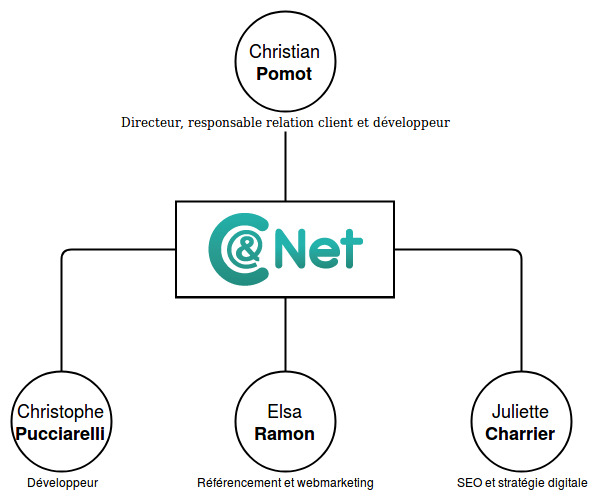
\includegraphics[scale=0.65]{Com&Net.jpg}
	\caption{organization of the Com\&Net company}
\end{figure}

\begin{figure}[p]
	\centering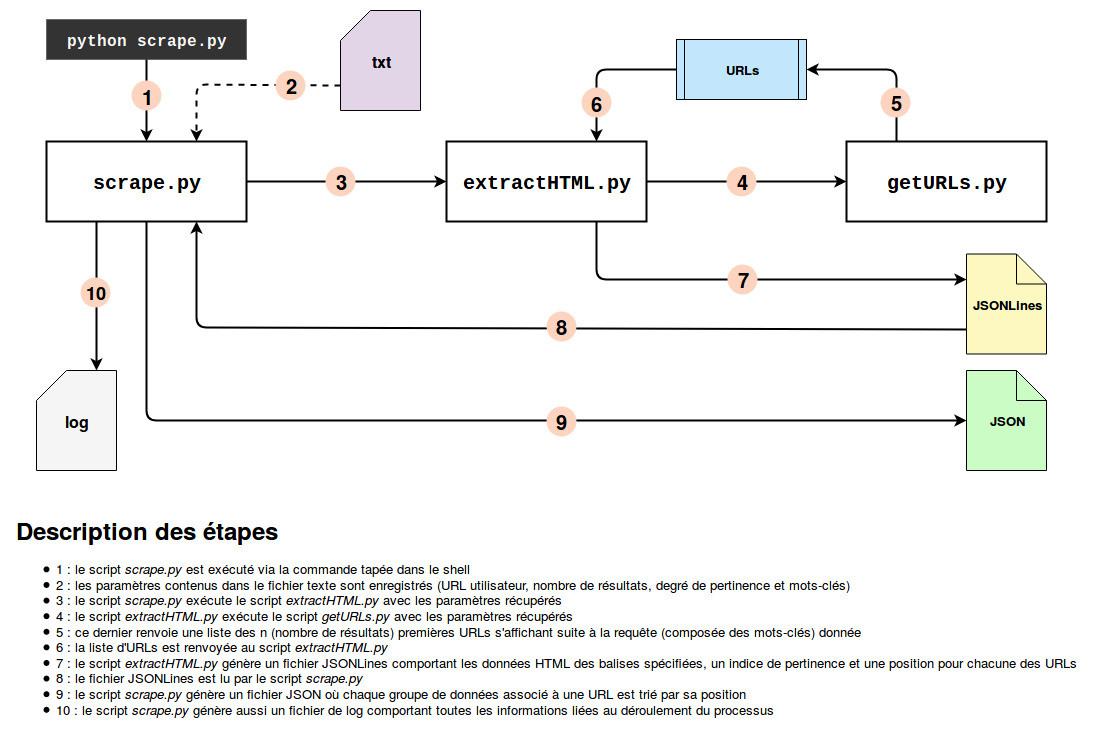
\includegraphics[scale=0.45]{architectureScraping.jpg}
	\caption{schematic representation of the architecture of the scraping engine}
\end{figure}

\begin{figure}[p]
	\centering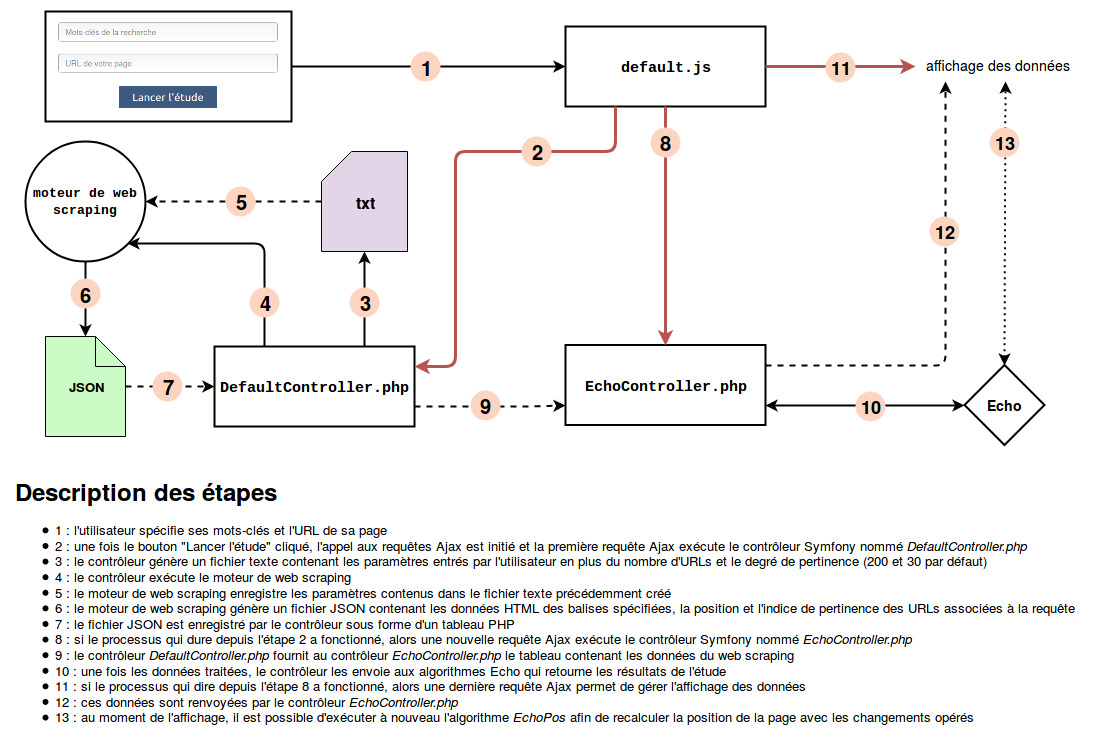
\includegraphics[scale=0.45]{architectureMachineLearning.jpg}
	\caption{schematic representation of the architecture of the Symfony project}
\end{figure}

\

\begin{figure}[p]
	\centering
	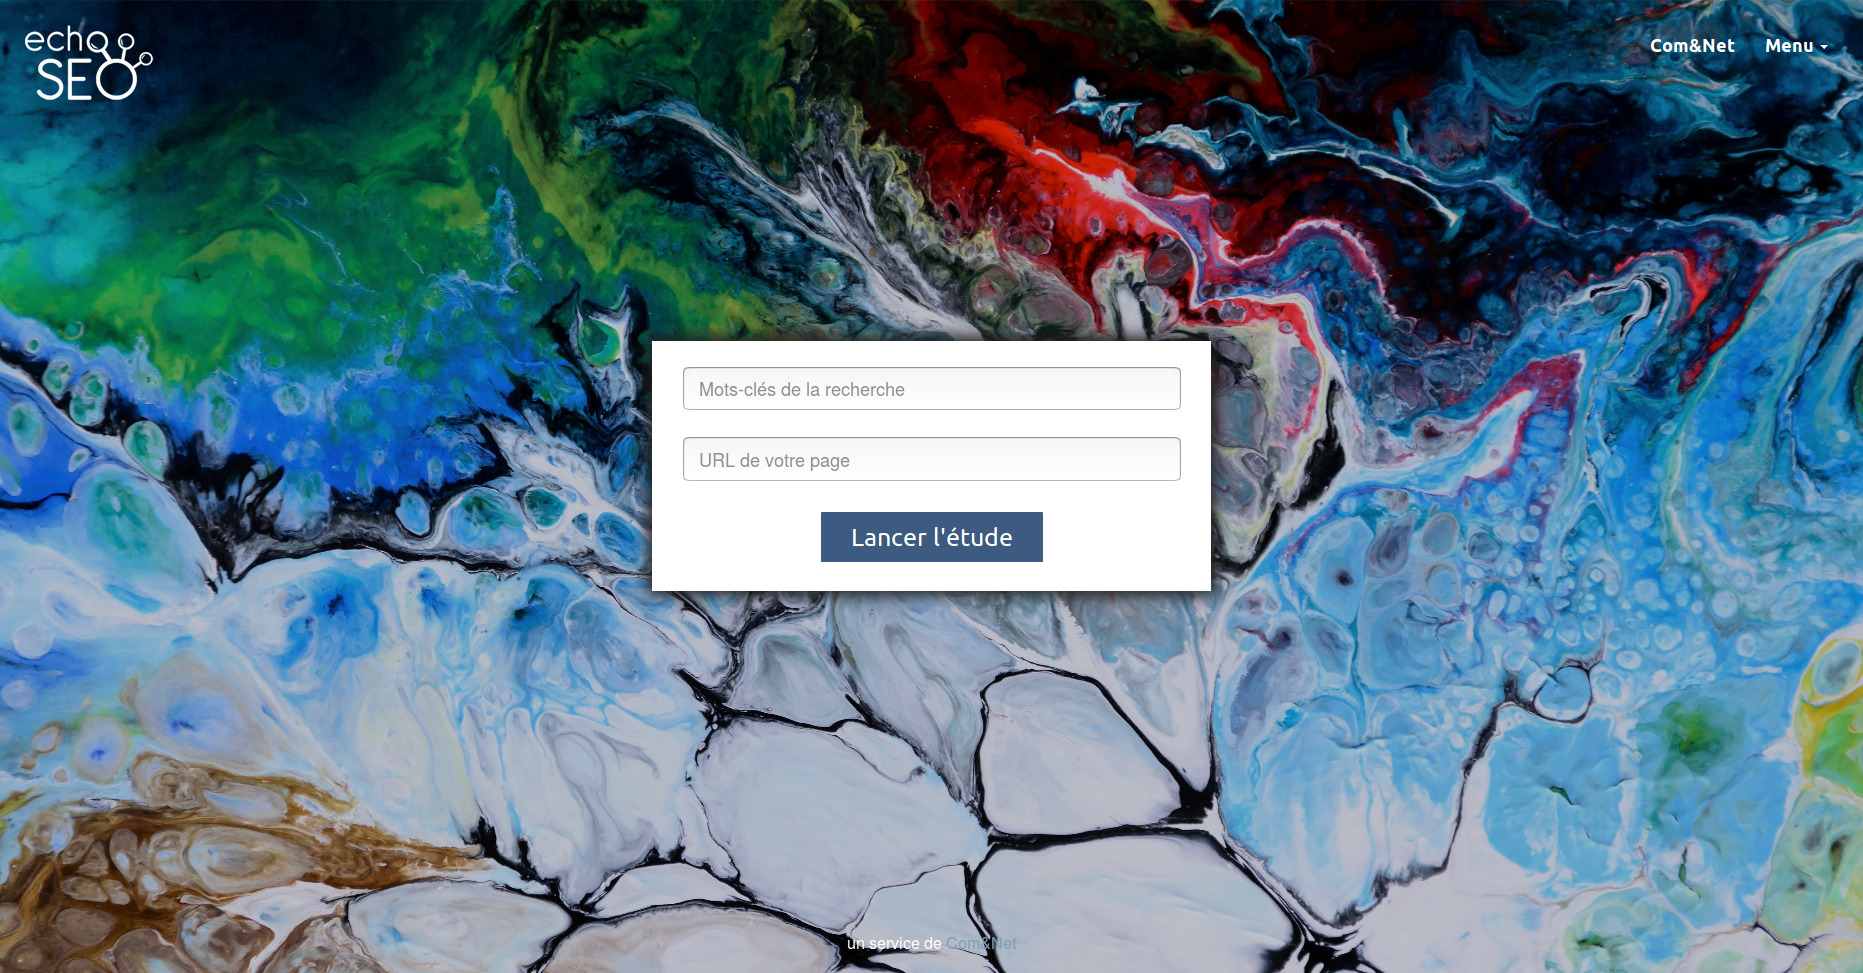
\includegraphics[scale=0.25]{ecranAccueil.jpg}
	\caption{screenshot of the home screen}
\end{figure}
\begin{figure}[p]
	\centering
	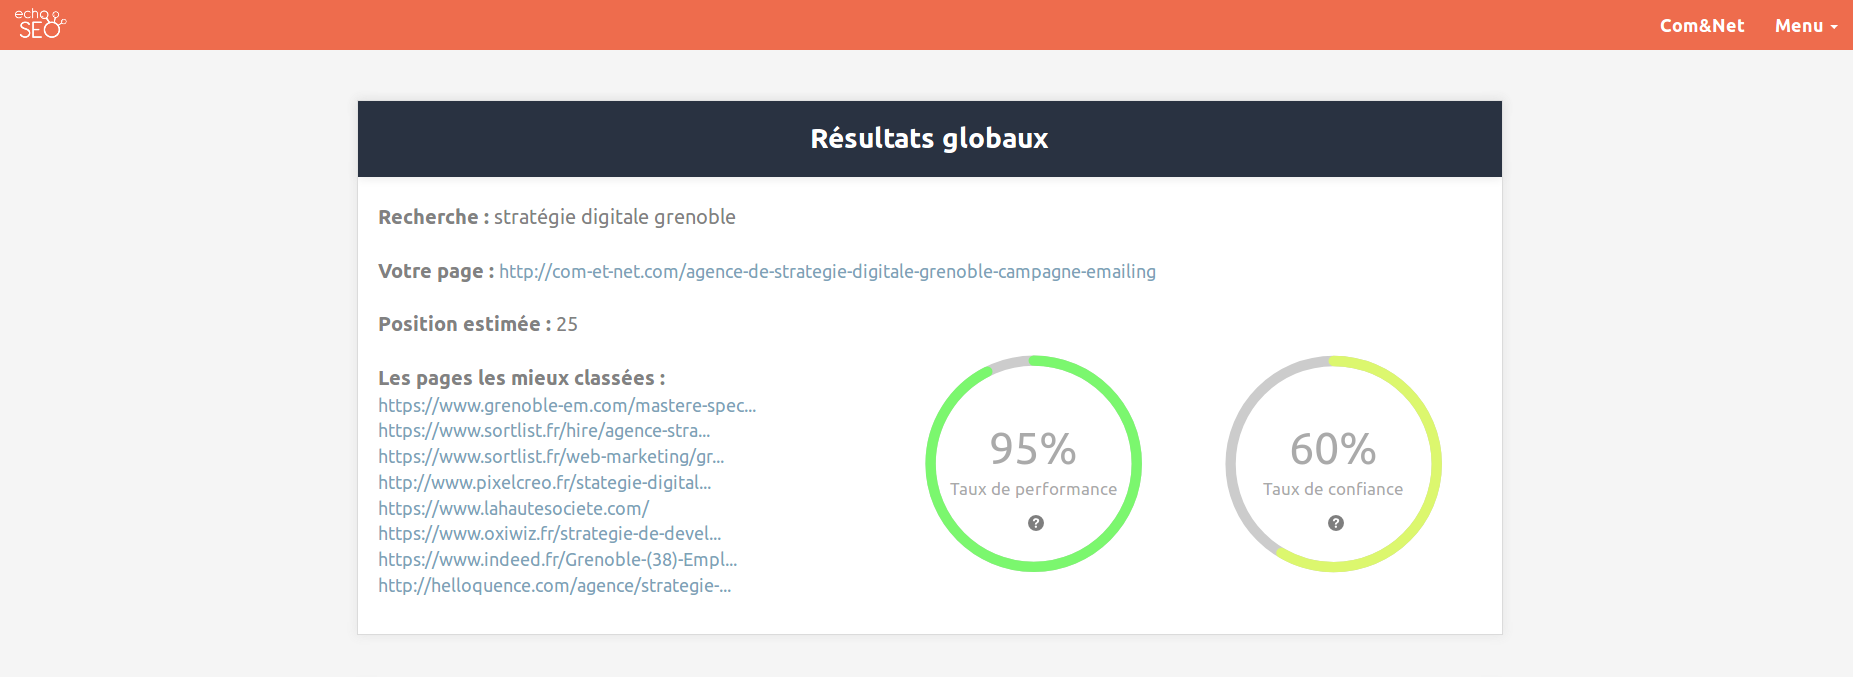
\includegraphics[scale=0.25]{hautDePage.png}
	\caption{screenshot of the top of the results page}
\end{figure}
\begin{figure}[p]
	\centering
	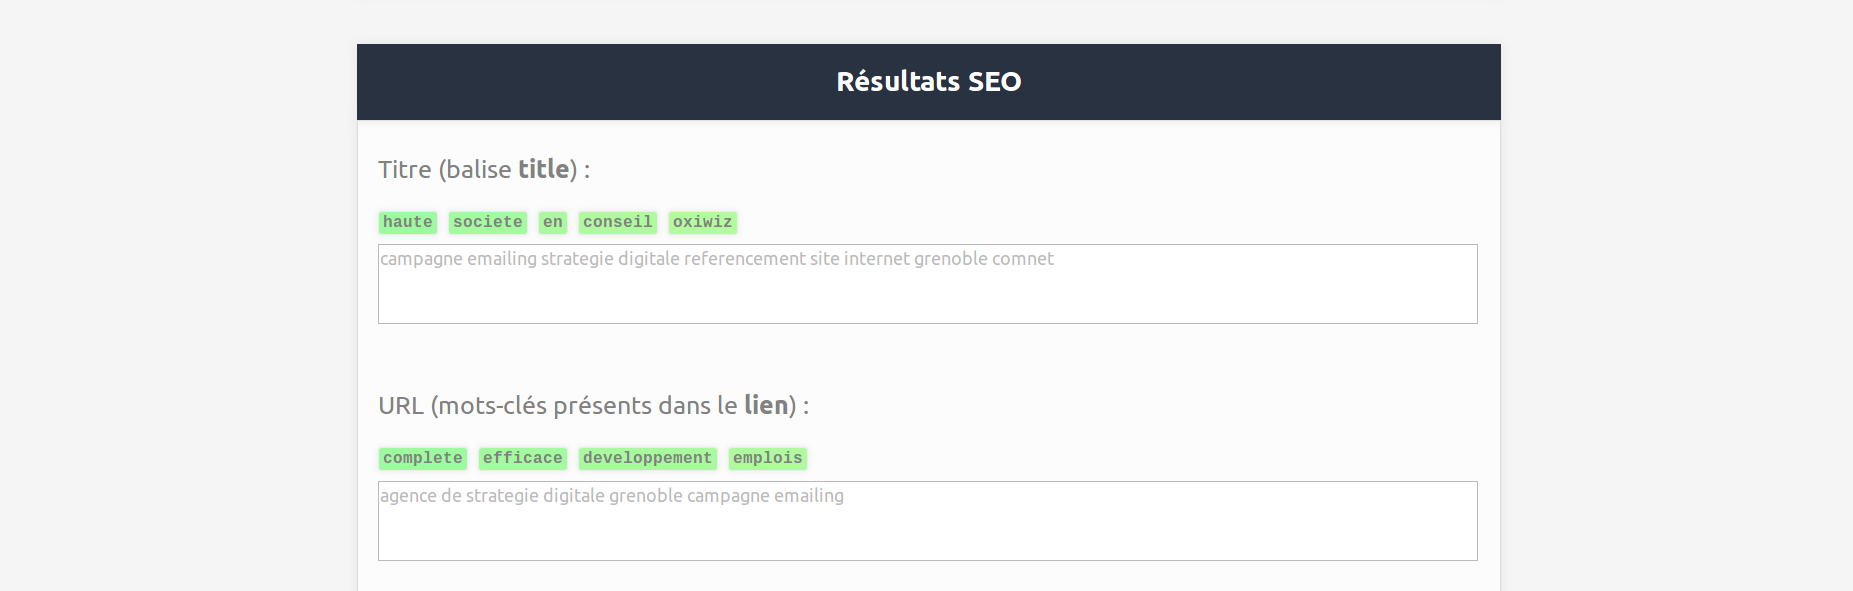
\includegraphics[scale=0.25]{milieuDePage.png}
	\caption{screenshot of the middle of the results page}
\end{figure}
\begin{figure}[p]
	\centering
	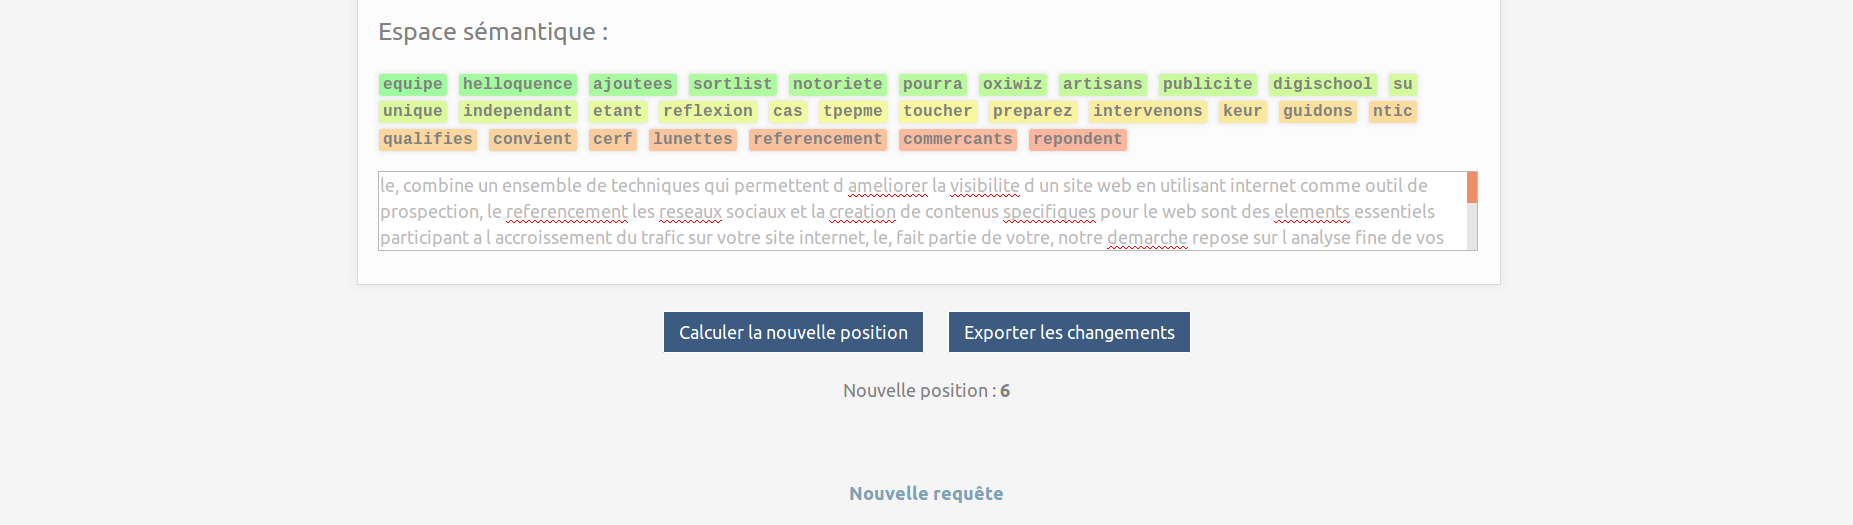
\includegraphics[scale=0.25]{basDePage.png}
	\caption{screenshot of the bottom of the results page}
\end{figure}

\

\newpage
\begin{figure}[p]
	\centering
	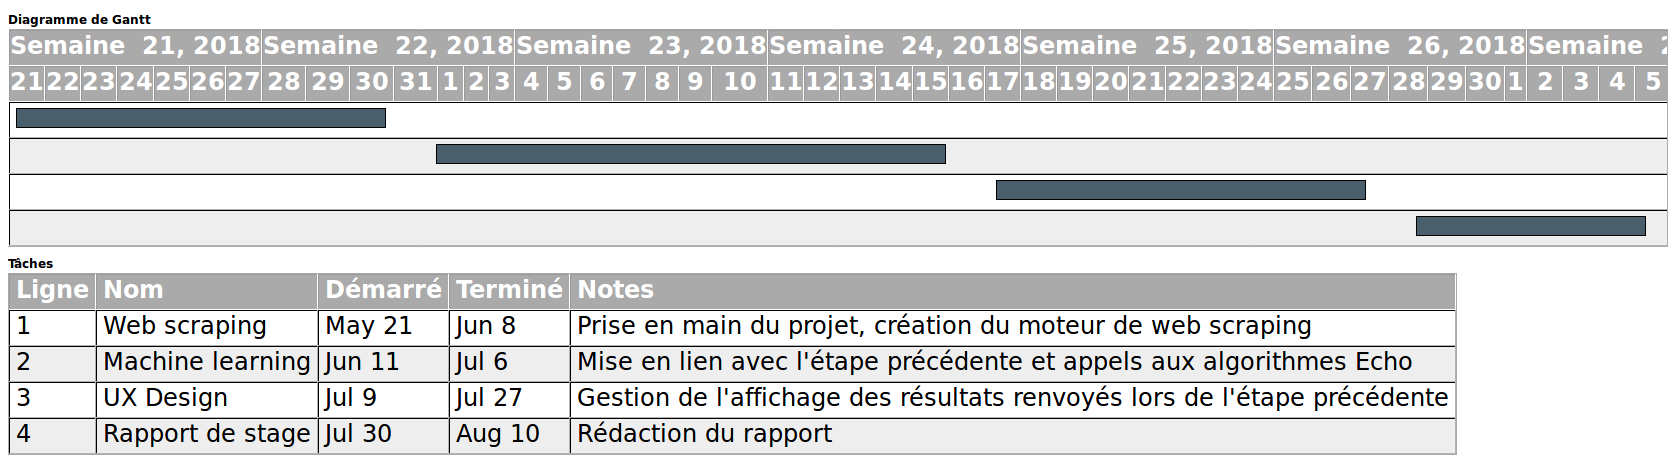
\includegraphics[scale=0.3]{gantt.png}
	\caption{Gantt chart}
\end{figure}

\end{appendices}

\end{document}